\section{Implementation}
\label{sec:imple}


\begin{figure*}[t!]
  \centering
  % 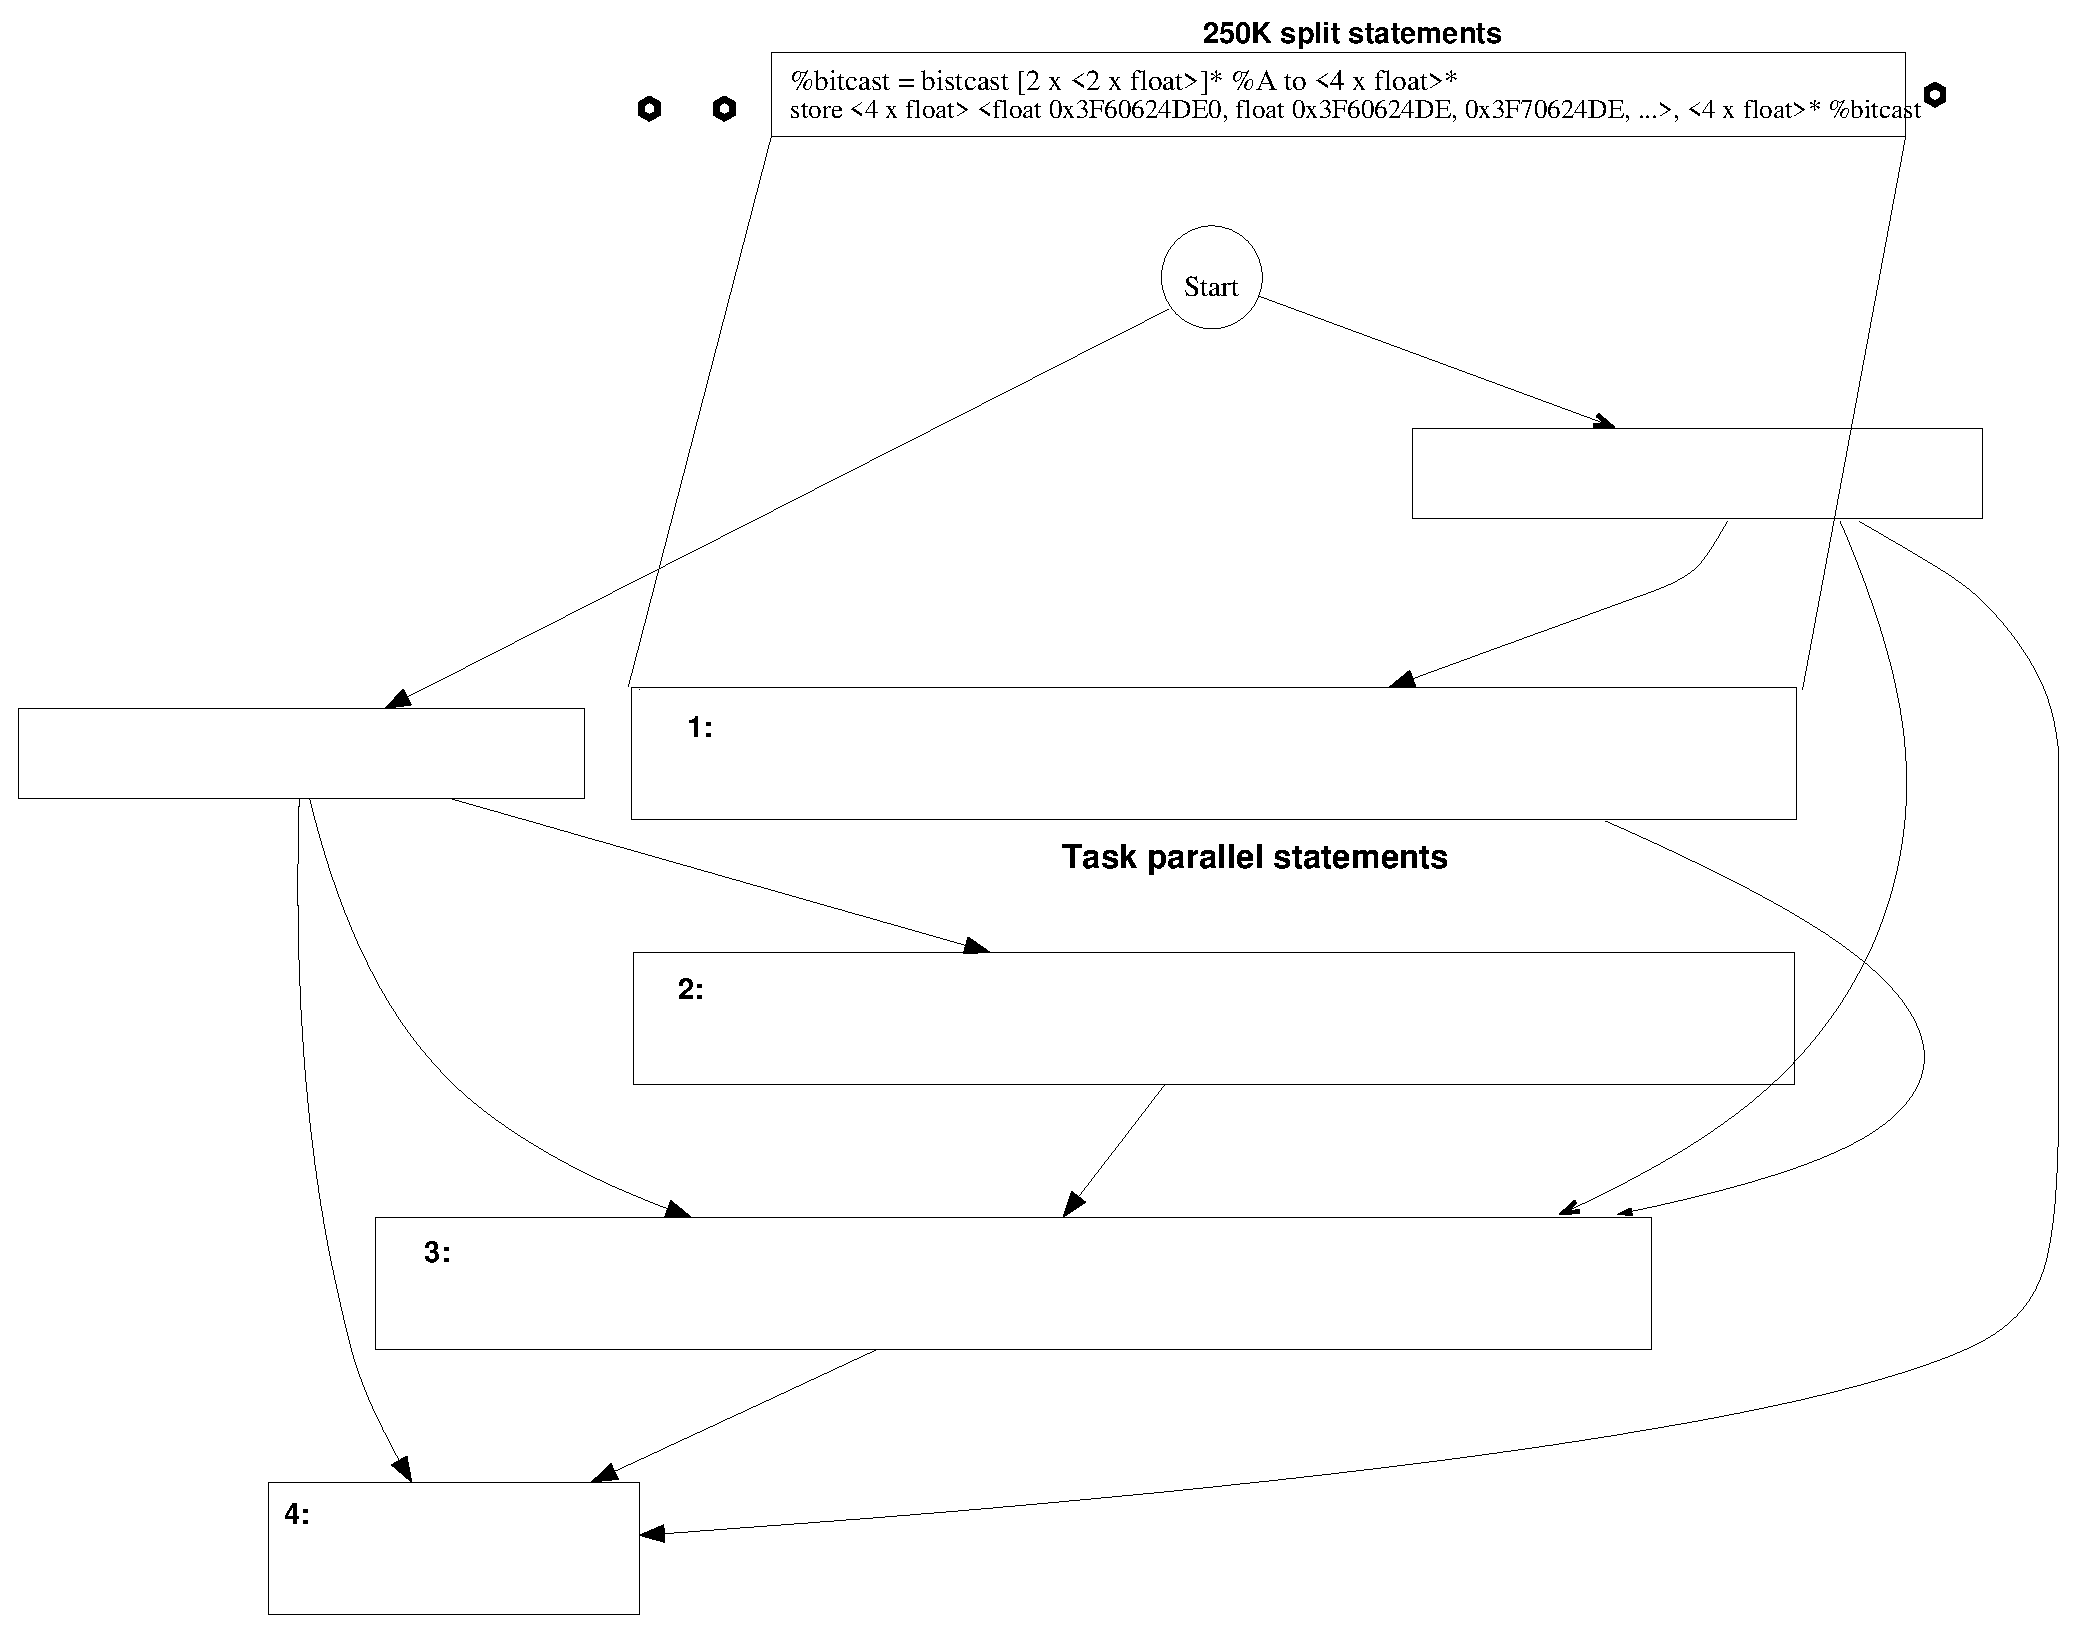
\includegraphics[scale=0.42]{./figures/jacobi2d}
  \scalebox{0.4}{\input{./figures/dendrogram.pstex_t}}
  \caption{The dendrogram for Figure~\ref{fig:res}}
  \label{fig:7}
\end{figure*}

We use the Metis~\cite{gkar95} graph partitioning library to implement
our partitioning algorithm. We are not tied to Metis and any other graph
partitioner such as Zoltan~\cite{kdev09} or Scotch~\cite{cche08} can be
used for implementing our algorithm. Herein, we describe how we used
Metis to implement the graph partitioning.

Metis is a graph partitioner, which implements K-way and recursive
bipartite graph partitioning. The weights on the graph nodes are
represented as constraints. Each graph node can have multiple-node
weights, representing different criteria. The edges between nodes can be
weighted themselves, but opposed to nodes, edges can only be decorated
with a single weight. Moreover, the unique point about Metis is that one
can use a concept called ``tp-weights'', which give weightage, to
different node constraints when performing load-balancing during K-way
or recursive graph partitioning. These are the only features of Metis
that we required when implementing our algorithm. Metis provides a
number of other features, which the readers can lookup in~\cite{gkar95}.

\subsection{Clustering the resource-graph}
\label{sec:clust-reso-graph}

First we describe the formation of the resource cluster graph shown in
Figure~\ref{fig:res}, given a resource-graph.

\begin{itemize}

% \item The task-graph in Figure~\ref{fig:1}, is represented as an
%   undirected graph in the Metis file format.

\item The resource-graph is represented in the Metis graph format. We
  represent the PEs capabilities as constraints of the nodes and the
  link's bandiwdths as communication volume on the edges.

\item We then construct our clustered structure (Figure~\ref{fig:res})
  by asking for a 2-way partition at each level of the $log_2|V_r|$
  height hierarchy. Metis partitions the graph by load balancing the
  constraints and performing a minimum edge cut. The number of
  partitions that Metis provides is bounded by $|V_r|/2$. Metis might
  provide fewer than $|V_r|/2$ partitions, if they lead to a better
  load-balance. In such a case, we continue with asking a 2-way
  partition at further levels of the hierarchy, but the height of the
  resultant hierarchical cluster is less than $log_2|V_r|$. Effective
  computation and communication costs are calculated at each stage using
  the formulation described in Section~\ref{sec:clustering-topology}.

\end{itemize}

\subsection{Partitoning the task-graph}
\label{sec:part-task-graph}

In partitioning the task graph, we need to balance the constraints on to
the available partitions. Metis offers the ability to load balance
multiple constraints on to different partitions based on the metric
\mbox{`tp-weight'}. We calculate the ratios between the capabilities of
different partitions and represent them as this metric in order to load
balance on to the available partitions. The steps followed are as
follows:

\begin{itemize}

\item We start at the top most level (level 3, Figure~\ref{fig:res}) in
  the resource-graph hierarchy, and request for the number of partitions
  equal to that of the child nodes at the next level, usually a 2-way
  partition.

\item The capabilities of the resource graph are represented as ratios
  for each of the constraint as the `tp-weight' metric when partitioning
  the task graph using Metis. For example, consider the partitioning
  onto the level 1 resource-graph in Figure~\ref{fig:res}. There are 4
  contracted nodes. We generate two sets of `tp-weights', with 2
  elements each, one for each of the node sets contracted to form the
  parent level (level-2, Figure~\ref{fig:res}). Each element in the set
  represents the MIPS count and the vector capacity of the underlying
  contracted node. Let us consider node \texttt{A2}, which is
  effectively the contraction of nodes \texttt{C1} and
  \texttt{A1}. Thus, the MIPS capacity element, of the `tp-weight' set
  for weight set for the nodes \texttt{C1} and \texttt{A1} are
  calculated as: {$\{C1^{MIPS}_{tpw} = R^{C1}_0/R^{C1}_0 + R^{A1}_0,
    A1^{MIPS}_{tpw} = R^{C1}_0/R^{C1}_0 + R^{A1}_0\}$}. Same is done to
  calculate the vector length capacity ratios. Since, the other two
  nodes \texttt{B1} and \texttt{D1} are contracted to form the second
  parent in level 2, \texttt{B2}, we end up with two sets of
  `tp-weights'.

\item As we go down on to each level we partition the task graph into
  smaller fine grained parts until we reach the lowest level. Note that
  the `tp-weight' sets are calculated for every level in the
  resource-graph hierarchy.

\item Finally, the entire task graph is partitioned into sub graphs
  where each of them are mapped onto a specific PE in the resource
  graph.

\end{itemize}


% \subsection{Load Balancing Multiple Constraints}

% Metis load balances constraints by minimizing the imbalance with that of
% an ideal value. It tries to acheive this by modifying the partitioning
% such that each consrtaint lies within certain imbalance from the ideal
% value. Since reaching an `optimal' solution is difficult (or in some
% cases impossible), it matches each of the constraint in
% \underline{order} until it finds a solution where all the constraints
% are matched within a certain tolerance level. Unfortunately, this causes
% the contraint to be matched with more and more imbalance as we move
% further, thereby giving priority to the first node constraint and then
% to the second and so on and so forth.

% In order to handle this, we chose an addition to our heuristic that
% checks whether we achieve the least imbalance in compute power in our
% partitions. This is done by clustering the nodes at each level based
% on all the possible permutations of the resource graph. After each
% clustering for a given permutation the imbalance in compute power is
% calculated as,

% \begin{equation}
% \begin{array}{c}
% desired_compute_power = total_compute_power / no_of_nodes;\\

% for each partition, for 1->n\\
% cp_n = sum( ( compute power of node ( R * R .. Rn ) ) -
% desired_compute_power )\\

% chosen partition = min( cp_n  )\\
% \end{array}
% \end{equation}

% We then pick the partition that was yielded with the minimum deviation
% in the compute power.

\subsection{The post pass}
\label{sec:post-pass}




%%% Local Variables: 
%%% mode: latex
%%% TeX-master: "bare_conf"
%%% End: 
